\section{Date: 2026-10-10}
\noindent \textbf{Series ID: MRTSIM4423XUSN} 

\noindent This series is titled Retail Inventories: Furniture, Home Furnishings, Electronics, and Appliance Stores and has a frequency of Monthly, End of Period. The units are Millions of Dollars and the seasonal adjustment is Not Seasonally Adjusted.The observation start date is 1992-01-01 and the observation end date is 2026-07-01.The popularity of this series is 1. \\ 

\noindent \textbf{Series ID: NENGPCERECGD} 

\noindent This series is titled Personal Consumption Expenditures: Goods: Durable Goods: Recreational Goods and Vehicles for New England BEA Region and has a frequency of Annual. The units are Millions of Dollars and the seasonal adjustment is Not Seasonally Adjusted.The observation start date is 1997-01-01 and the observation end date is 2025-01-01.The popularity of this series is 1. \\ 

\subsection{Raw Regression}
\noindent Regresses the two series against each other directly. A significant result here can come just as easily from both series sharing a long-run trend as from any real relationship.

\begin{center}
\begin{tabular}{lclc}
\toprule
\textbf{Dep. Variable:}              & value\_fred\_NENGPCERECGD & \textbf{  R-squared:         } &     0.273   \\
\textbf{Model:}                      &            OLS            & \textbf{  Adj. R-squared:    } &     0.246   \\
\textbf{Method:}                     &       Least Squares       & \textbf{  F-statistic:       } &     10.15   \\
\textbf{Date:}                       &      Sat, 10 Oct 2026     & \textbf{  Prob (F-statistic):} &  0.00363    \\
\textbf{Time:}                       &          16:26:49         & \textbf{  Log-Likelihood:    } &   -287.52   \\
\textbf{No. Observations:}           &               29          & \textbf{  AIC:               } &     579.0   \\
\textbf{Df Residuals:}               &               27          & \textbf{  BIC:               } &     581.8   \\
\textbf{Df Model:}                   &                1          & \textbf{                     } &             \\
\textbf{Covariance Type:}            &         nonrobust         & \textbf{                     } &             \\
\bottomrule
\end{tabular}
\begin{tabular}{lcccccc}
                                     & \textbf{coef} & \textbf{std err} & \textbf{t} & \textbf{P$> |$t$|$} & \textbf{[0.025} & \textbf{0.975]}  \\
\midrule
\textbf{const}                       &   -1.476e+04  &     1.06e+04     &    -1.391  &         0.176        &    -3.65e+04    &     7005.905     \\
\textbf{value\_fred\_MRTSIM4423XUSN} &       1.2545  &        0.394     &     3.185  &         0.004        &        0.446    &        2.063     \\
\bottomrule
\end{tabular}
\begin{tabular}{lclc}
\textbf{Omnibus:}       &  8.896 & \textbf{  Durbin-Watson:     } &    0.276  \\
\textbf{Prob(Omnibus):} &  0.012 & \textbf{  Jarque-Bera (JB):  } &    7.446  \\
\textbf{Skew:}          &  1.189 & \textbf{  Prob(JB):          } &   0.0242  \\
\textbf{Kurtosis:}      &  3.715 & \textbf{  Cond. No.          } & 3.03e+05  \\
\bottomrule
\end{tabular}
%\caption{OLS Regression Results}
\end{center}

Notes: \newline
 [1] Standard Errors assume that the covariance matrix of the errors is correctly specified. \newline
 [2] The condition number is large, 3.03e+05. This might indicate that there are \newline
 strong multicollinearity or other numerical problems.

\begin{figure}
\centering
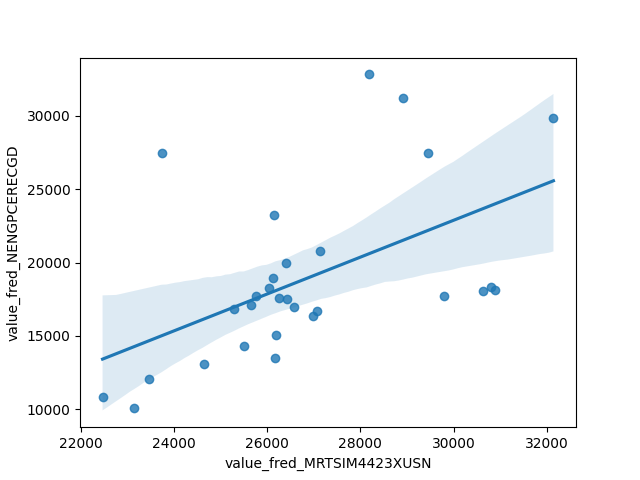
\includegraphics[scale = 0.9]{plots/plot_2026-10-10.png}
\caption{Raw Regression Plot for 2026-10-10}
\end{figure}
\newpage
\subsection{Detrended Regression}
\noindent Regresses the residuals of each series after removing its own linear time trend, so a shared trend can no longer drive the result on its own. A relationship that stays significant here is better evidence of a genuine link between the two series.

\begin{center}
\begin{tabular}{lclc}
\toprule
\textbf{Dep. Variable:}                         & value\_fred\_NENGPCERECGD\_detrended & \textbf{  R-squared:         } &     0.208   \\
\textbf{Model:}                                 &                 OLS                  & \textbf{  Adj. R-squared:    } &     0.179   \\
\textbf{Method:}                                &            Least Squares             & \textbf{  F-statistic:       } &     7.089   \\
\textbf{Date:}                                  &           Sat, 10 Oct 2026           & \textbf{  Prob (F-statistic):} &   0.0129    \\
\textbf{Time:}                                  &               16:26:49               & \textbf{  Log-Likelihood:    } &   -264.85   \\
\textbf{No. Observations:}                      &                    29                & \textbf{  AIC:               } &     533.7   \\
\textbf{Df Residuals:}                          &                    27                & \textbf{  BIC:               } &     536.4   \\
\textbf{Df Model:}                              &                     1                & \textbf{                     } &             \\
\textbf{Covariance Type:}                       &              nonrobust               & \textbf{                     } &             \\
\bottomrule
\end{tabular}
\begin{tabular}{lcccccc}
                                                & \textbf{coef} & \textbf{std err} & \textbf{t} & \textbf{P$> |$t$|$} & \textbf{[0.025} & \textbf{0.975]}  \\
\midrule
\textbf{const}                                  &     1.57e-10  &      430.842     &  3.64e-13  &         1.000        &     -884.015    &      884.015     \\
\textbf{value\_fred\_MRTSIM4423XUSN\_detrended} &       0.5177  &        0.194     &     2.663  &         0.013        &        0.119    &        0.917     \\
\bottomrule
\end{tabular}
\begin{tabular}{lclc}
\textbf{Omnibus:}       &  1.587 & \textbf{  Durbin-Watson:     } &    0.389  \\
\textbf{Prob(Omnibus):} &  0.452 & \textbf{  Jarque-Bera (JB):  } &    1.285  \\
\textbf{Skew:}          &  0.499 & \textbf{  Prob(JB):          } &    0.526  \\
\textbf{Kurtosis:}      &  2.742 & \textbf{  Cond. No.          } & 2.22e+03  \\
\bottomrule
\end{tabular}
%\caption{OLS Regression Results}
\end{center}

Notes: \newline
 [1] Standard Errors assume that the covariance matrix of the errors is correctly specified. \newline
 [2] The condition number is large, 2.22e+03. This might indicate that there are \newline
 strong multicollinearity or other numerical problems.

\begin{figure}
\centering
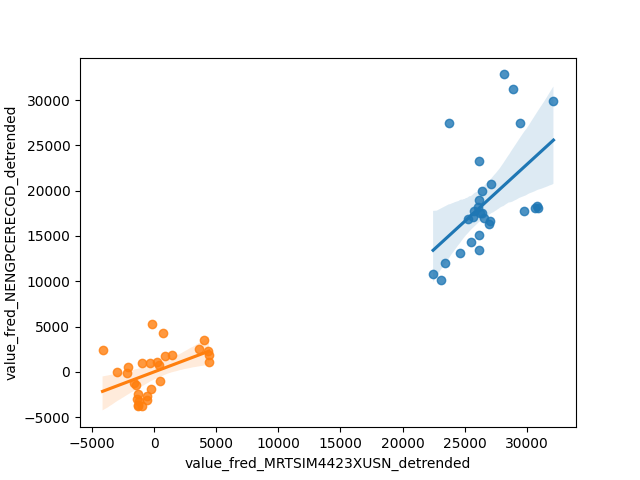
\includegraphics[scale = 0.9]{plots/plot_2026-10-10_detrended.png}
\caption{Detrended Regression Plot for 2026-10-10}
\end{figure}
\newpage
